% Format :  Latex2e
\documentclass[11pt]{article}
\usepackage{amsmath}
\usepackage{amssymb}
\usepackage{enumerate}
\usepackage{boxedminipage}
\usepackage{float}
\usepackage{graphicx}
\usepackage{url}
\usepackage{verbatim}
%\documentstyle{article}
\setlength{\oddsidemargin}{0.in} \setlength{\evensidemargin}{0.in}
\setlength{\textwidth}{6.50in} \setlength{\topmargin}{-.50in}
\setlength{\textheight}{9in} \setlength{\headheight}{.1in}
\setlength{\headsep}{.3in} \setlength{\rightskip}{0pt plus .5fil}

\begin{document}
\restylefloat{table}
\thispagestyle{empty}
\pagestyle{plain}
%
\begin{center}
{\bf Tips N' Tricks: \\ 
Using Stata in Terminal or Batch Mode}
\end{center}

\noindent Here is another advanced tip or trick. For those who are programmers or who know how to work on the "command line". Stata, similar to R, is really a set of background programs that also run in a terminal (Unix/Linux, i.e. Mac), or Command Prompt (Windows, similar to DOS). The Stata setup that you normally see is just a GUI, Graphical User Interface, which puts a pretty coat of paint on top of the underlying program. You can use this to your advantage in several ways.

\section{Run Stata in terminal mode like a real programmer}

\noindent One advantage of running Stata in the terminal on Mac/Linux, or the command prompt on Windows, is that it is much less resource intensive. If you are doing calculations that really tax your computer's RAM and Processing Power, a text only terminal will save more computing resources for the underlying processes. Another advantage is it's just cool and you look like a real programmer. Finally, a third advantage is you can use your favorite text editor and send code directly to the terminal. I recommend Sublime Text 3 on Mac/Windows/Linux, or NotePad++ on Windows. It's also often faster to work this way. \\
\\
\noindent The disadvantage to running Stata in a terminal window is that you have no graphics capabilities to view your graphs, without some jumping through some complicated hoops. So essentially, you can create the graphs and export or save them, and view them later. You also have no ability to use the data browser. But you can use commands to view parts of your data in text mode in the browser.

\begin{figure}[htbp]
\begin{center}
 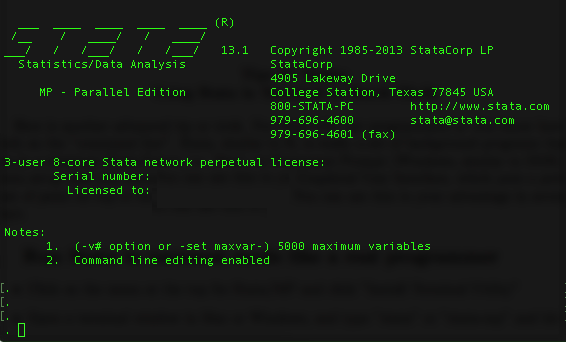
\includegraphics[clip=true,width=.5\textwidth,keepaspectratio]{stataterminal.png}
\caption{Stata 13 running in Terminal Mode on a Mac.}
\label{default}
\end{center}
\end{figure}

\noindent To use Stata in the terminal, follow these steps.
\begin{itemize}
\item Click on the menu at the top for Stata/MP and click ``Install Terminal Utility''.
\item Open a terminal window in Mac or Windows, and type \verb!stata! or \verb!stata-mp! and hit enter.
\item Install and customize a text editor such as Sublime 3 to be able to send code to the terminal.
\item You can also navigate to the location of a \verb!.do! file in Stata terminal with \verb!cd!, and type \verb!do name_of_do_file.do!
\end{itemize}

\section{Run Stata in batch mode for maximal resource efficiency\protect\footnote{Remember to always create log files, in both terminal mode and especially in batch mode, so you can review your output for errors later!}}

\noindent If you have already perfected your .do file, and perhaps tried your analyses or manipulations on a small section of your data, but now you want to run it in a way that completely minimizes resource use, you can go one step further and even get rid of terminal text by running it in batch mode. You won't see any cool matrix-like scrolling text in your terminal window, just a blinking cursor. But your computer or server will be running everything quietly in the background. You can even run multiple files this way. \\

\noindent To run Stata in batch mode:
\begin{itemize}
\item Open a terminal or command prompt window
\item In Unix/Linux type \verb!stata -b do filename &!
\item In Windows, type \verb!C:\Program Files\Stata14\StataMP" /b do c:\data\bigjob.do!
\item You can also write Unix/Linux \verb!.sh! files or Windows \verb!.bat! batch files to run a bunch of Stata batch programs in a row. This is convenient when you have a large number of \verb!.do! files to run for your project.
\end{itemize}

\noindent For more information, see here:\\
\url{http://www.stata.com/support/faqs/unix/batch-mode/} \\
for Unix/Linux, or here:\\
\url{http://www.stata.com/support/faqs/windows/batch-mode/}\\
for Windows.

\section{Terminal shell and programs from within Stata and vice versa}

\noindent Sometimes you might run into some limitations with Stata's abilities. Whether you are running Stata in terminal mode, or in GUI mode (normal), you can always call terminal commands from within your Stata .do files so you can access the power of the terminal/command line and other programs such as R or Python. Similarly, you can sometimes call Stata to run commands from within other scriptable programs such as R. This is helpful so that you can integrate all of your code into one, automatically reproducible file and not have to manually stop and start other programs. Just remember that you will sometimes need to export files into other formats readable by other programs, and them import output files back into Stata as necessary.\footnote{Note: You must use the proper code Unix/Linux/Windows for the operating system you are working on.} \\

\noindent Here are some examples of using the Stata shell:
\begin{itemize}
\item Typing \verb!shell! in Stata's console, or a \verb!.do! file will open a terminal window.
\item Typing \verb!shell erase *.smcl! on a Windows computer will tell the windows command line to erase all log files in the current folder, and then continue return to Stata
\item Typing \verb!shell rm *.smcl! on a Unix(Mac)/Linix computer will do the same
\item Typing an exclamation mark \verb!!! at the beginning of the line is the same as typing \verb!shell!
\item If you have multiple lines of code to run, you need to put a \verb!!! or \verb!shell! at the beginning of each line. But if your code is too long, you can instead write a separate file of code and call that to be run with the shell from Stata.
\item For some programs, such as R, there are dedicated, user-written, add-on packages for Stata that give even better functionality. For example, if you want to run a chunk of R code, you could use the Stata program, RSOURCE, by typing \verb!ssc install rsource!. More info is located here: \url{https://ideas.repec.org/c/boc/bocode/s456847.html}
\item In reverse direction, if you are doing most of your work in R or another program, there are ways to run some quick Stata commands from there either with add-on packages, or by using that program's terminal/shell capabilities to run a Stata \verb!.do! file.
\end{itemize}

\noindent For more information, see here:\\
\url{http://www.stata.com/manuals13/dshell.pdf}

\section{Mouse jigglers and server timeouts}

\noindent If you are using some of the tips above, especially "batch mode", it is very likely that you have an enormous dataset, or very large calculations that are running very slowly. You are probably using these tips to speed things up on processes that take hours, or days to run. As a result, you may gain some speed by running things on a server, such as that of the PRC. But then, you have the problem of automatic log-outs. The PRC and UT Stats Server used to allow batch-processing where you could send a code file and get an email the next day when your results were done. This has not been allowed for the past several years. Instead, they have a 2 hour log-out time when on campus, and a 1/2 hour logout time when off-campus. One way to get around this is to change your personal computer settings to never go to sleep, and use a program called a mouse-jiggler that jiggles your cursor every 2 minutes to trick the server into thinking you are still connected. I have personally left my computer running batch processes for 3 or 4 days with this method. \\

\noindent Here is a free mouse jiggler for Mac:\\
\url{http://www.sticksoftware.com/software/Jiggler.html}\\
\\
\noindent And here is a free one for Windows:\\
\url{https://mousejiggler.codeplex.com}

\section{Why the hell would I bother to do any of this stuff?}

\noindent Aside from the ``geek factor'', speed, computer resource efficiency, integration of Stata with other programs, and enhanced capabilities, there is are two very important reasons to consider these methods:

\begin{itemize}
\item {\bf\Large REPLICABILITY:} Replicability implies that your research can be replicated. By making the code for your analyses integrated into a coherent, organized, and integrated set of script files, you increase the chances that both you and future researchers potentially interested in replicating your work will be able to do so, perform the same exact steps in the same order, and ultimately arrive at exactly the same results. This is an important part of quantitative research since, if you cannot replicate your exact results with the very same data, then they are questionable. Along these lines, whenever possible, it is preferable to ``code'' changes to your data when you are cleaning and organizing it, even if learning how to do so is more tedious. The advantage is obvious, because any changes you make manually to the data with a point-n-click program such as Microsoft Excel will be difficult to replicate, and will leave no record of the changes you made.
\item {\bf\Large REPRODUCIBILITY:} Reproducibility goes one very important step further than replicability, taking your entire research project from start to finish, from raw data, through data cleaning and organization, through data analyses, drafting of an article, creation and insertion of tables, charts, and graphs, insertion of footnotes, citations, and bibliography, and finally creation of a final draft of your article. Complete ``reproducibility'' is difficult, though not impossible with Stata, and requires some outside tools and languages such as \LaTeX or Markdown. It is much easier to achieve with some integrated tools in R. I will leave the conversation about ``reproducibility'' for another day. But suffice it to say that the ``replicability'' techniques for integrating Stata with other programming tools shared in this document bring you much closer to ``reproducible'' research. For now, just imagine what it would be like if you could press one button, or type one line of code, and could perfectly reproduce a final draft of your article including every step along the process. This is a common gold-standard in hard sciences research, but not so much in social sciences.
\end{itemize}

\noindent Here is a very opinionated article about the differences between ``replicability'' and ``reproducibility'':\\
\url{https://core.ac.uk/download/files/21/107703.pdf}



\end{document}
